%%% Preamble
\documentclass[paper=a4, fontsize=11pt]{scrartcl}
\usepackage[T1]{fontenc}
\usepackage{fourier}

\usepackage[english]{babel}															% English language/hyphenation
\usepackage[protrusion=true,expansion=true]{microtype}	
\usepackage{amsmath,amsfonts,amsthm} % Math packages
\usepackage[pdftex]{graphicx}	
\usepackage{url}
\usepackage{subcaption}
\usepackage{comment}
\usepackage{hyperref}

%%% Custom sectioning
\usepackage{sectsty}
\allsectionsfont{\centering \normalfont\scshape}


%%% Custom headers/footers (fancyhdr package)
\usepackage{fancyhdr}
\pagestyle{fancyplain}
\fancyhead{}											% No page header
\fancyfoot[L]{}											% Empty 
\fancyfoot[C]{}											% Empty
\fancyfoot[R]{\thepage}									% Pagenumbering
\renewcommand{\headrulewidth}{0pt}			% Remove header underlines
\renewcommand{\footrulewidth}{0pt}				% Remove footer underlines
\setlength{\headheight}{13.6pt}


%%% Equation and float numbering
\numberwithin{equation}{section}		% Equationnumbering: section.eq#
\numberwithin{figure}{section}			% Figurenumbering: section.fig#
\numberwithin{table}{section}				% Tablenumbering: section.tab#


%%% Maketitle metadata
\newcommand{\horrule}[1]{\rule{\linewidth}{#1}} 	% Horizontal rule

\title{
		%\vspace{-1in} 	
		\usefont{OT1}{bch}{b}{n}
		\normalfont \normalsize \textsc{Universidad Católica San Pablo - Ciencia de la Computación} \\ [25pt]
		\horrule{0.5pt} \\[0.4cm]
		\huge Pruebas sobre el comportamiento de la memoria caché \\
		\horrule{2pt} \\[0.5cm]
}


\author{Berly Esleider Vica Argandoña}

\date{}

%%% Begin document
\begin{document}
\maketitle
\section{Introducción}
Se implentaron los algoritmos de multiplicación de matrices en su versión clásica de 3 bucles anidados y la multiplicación de matrices por bloques, con el objetivo de comparar el comportamiento de la memoria caché, el código se encuentra \href{https://github.com/TKgitmode/Paralela/tree/main/Laboratorio1}{aquí}.

\section{Implementaciones}
Se usaron matrices cuadradas para hacer las comparaciones de tamañp 100, 500, 1000 y 2000. Los programas fueron programados en c++, se usaron las herramientas \textit{valgrind} y \textit{kcachegrind} para obtener una evaluación mas precisa de su desempeño en términos de caché misses.
\subsection{Multiplicación de Matrices Clásica}

\begin{comment}
\begin{itemize}
    \item Filtro: Aquello que discrimina elementos indeseables de un conjunto. En sistemas de control, un filtro es aquel que discrimina determinadas frecuencias de una señal eléctrica que pasa por él.
    \item Proceso: conjunto de actividades que se realizan bajo ciertas circunstancias y con un fin determinado.
\end{itemize}
\end{comment}

\begin{figure}[!h]
  \centering
  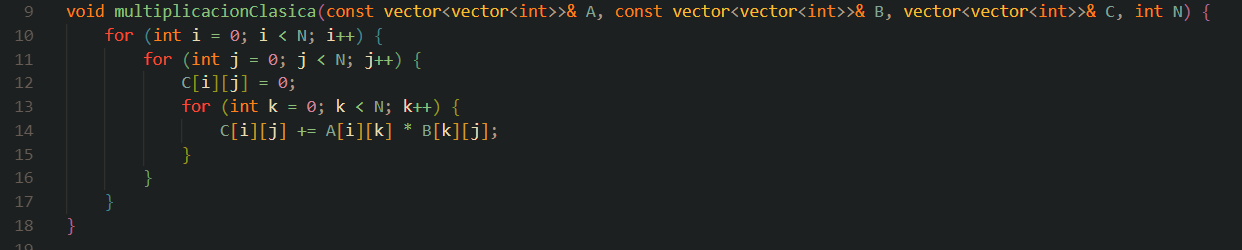
\includegraphics[width=\linewidth]{figures/matrizClasica1.png}
  \caption{Multiplicación de Matrices Clásica}
  \label{fig:1}
\end{figure}

\begin{figure}[!h]
  \centering
  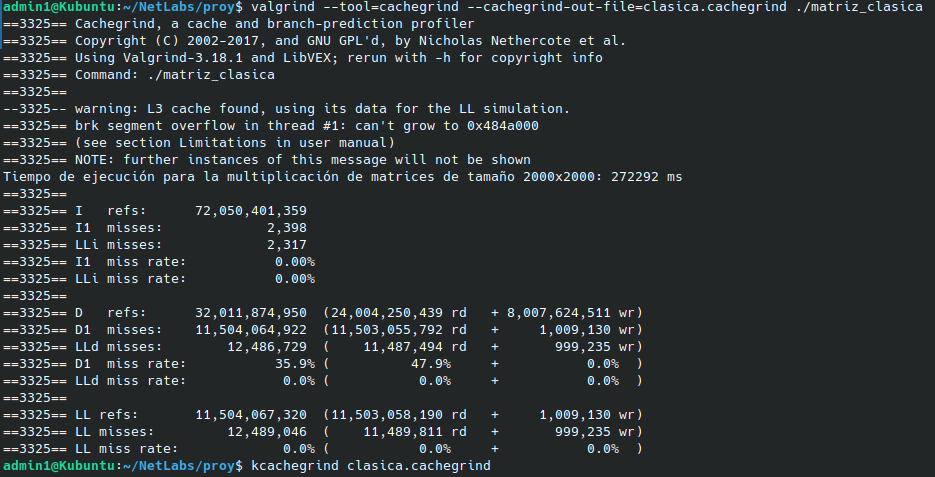
\includegraphics[width=\linewidth]{figures/clasica2.png}
  \caption{Valgrind}
  \label{fig:2}
\end{figure}

\begin{figure}[!h]
  \centering
  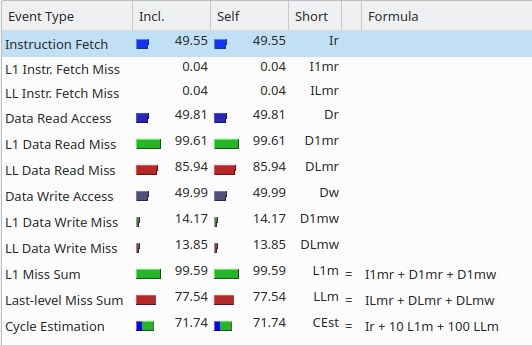
\includegraphics[width=\linewidth]{figures/clasica3.png}
  \caption{Kcachegrind}
  \label{fig:3}
\end{figure}

Al ejecutar el código con las herramientas \textit{Valgrind} y \textit{Kcachegrind} tenemos que:
\begin{enumerate}
    \item Para una matriz de 100x100, el tiempo que demora en hacer la multiplicación es \textit{8.9759 ms}.
    \item Para una matriz de 500x500, el tiempo que demora en hacer la multiplicación es \textit{1110.85 ms}.
    \item Para una matriz de 1000x1000, el tiempo que demora en hacer la multiplicación es \textit{9294.8 ms}.
    \item Para una matriz de 2000x2000, el tiempo que demora en hacer la multiplicación es \textit{102779.8 ms}.
    \item Tiene una complejidad de O($n^3$\hspace{-1mm} ).
\end{enumerate}

\subsection{Multiplicación de Matrices por Bloques}

\begin{figure}[!h]
  \centering
  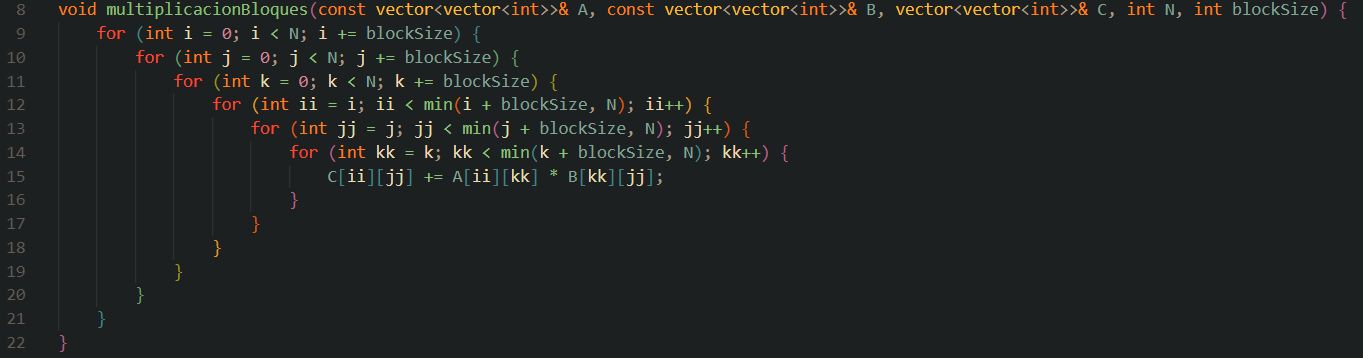
\includegraphics[width=\linewidth]{figures/multiBloques1.png}
  \caption{Multiplicación de Matrices por Bloques}
  \label{fig:4}
\end{figure}

Al ejecutar el código con las herramientas \textit{Valgrind} y \textit{Kcachegrind} tenemos que:
\begin{figure}[!h]
  \centering
  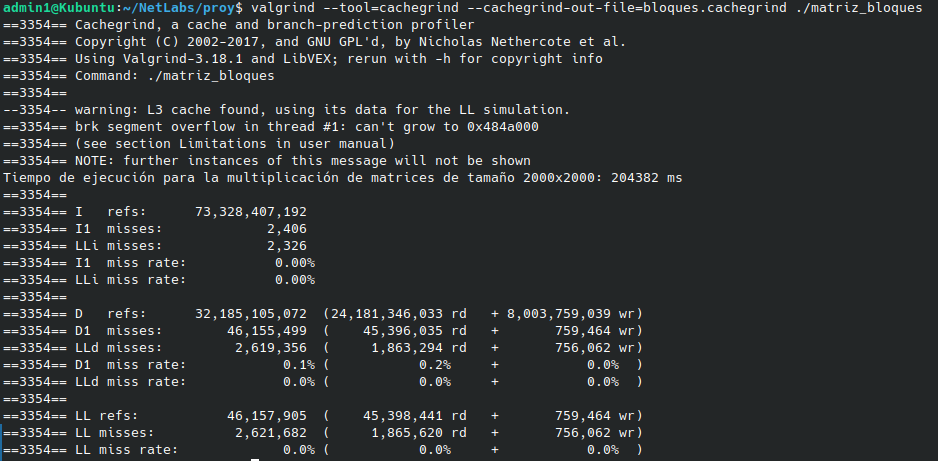
\includegraphics[width=\linewidth]{figures/bloques2.png}
  \caption{Valgrind}
  \label{fig:5}
\end{figure}

\begin{figure}[!h]
  \centering
  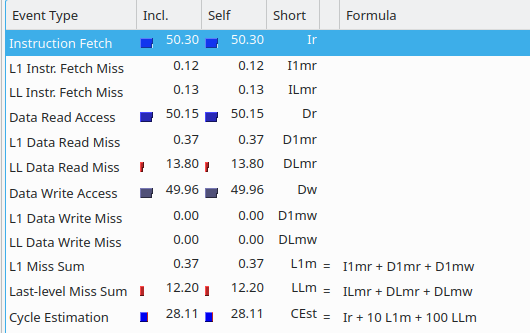
\includegraphics[width=\linewidth]{figures/bloques3.png}
  \caption{Kcachegrind}
  \label{fig:6}
\end{figure}

\begin{enumerate}
    \item Para una matriz de 100x100, el tiempo que demora en hacer la multiplicación es \textit{11.4584 ms}.
    \item Para una matriz de 500x500, el tiempo que demora en hacer la multiplicación es \textit{1347.52 ms}.
    \item Para una matriz de 1000x1000, el tiempo que demora en hacer la multiplicación es \textit{10650 ms}.
    \item Para una matriz de 2000x2000, el tiempo que demora en hacer la multiplicación es \textit{87166.5 ms}.
    \item Tiene una complejidad de O($n^3$\hspace{-1mm} ).
\end{enumerate}

\section{Comparativa del Desempeño} 
Recolectamos los siguientes datos comparando las figuras \figurename~\ref{fig:3} correspondiente a la multiplicación de matrices clásica y \figurename~\ref{fig:6} correspondiente a la multiplicación de matrices por bloques:
\begin{itemize}
    \item Con respecto a \textit{L1 Data Read Miss} la multiplicación por bloques es de \textit{0.37} a comparación del \textit{99.61} en el caso de la multiplicación de matrices clásica.
    \item Con respecto a \textit{LL Data Read Miss} la multiplicación por bloques es de \textit{13.80} a comparación del \textit{85.94} en el caso de la multiplicación de matrices clásica.
    \item Con respecto a \textit{Data Write Access} la multiplicación por bloques es de \textit{49.96} a comparación del \textit{49.99} en el caso de la multiplicación de matrices clásica.
    \item Con respecto a \textit{L1 Data Write Miss} la multiplicación por bloques es de \textit{0.0} a comparación del \textit{14.17} en el caso de la multiplicación de matrices clásica.
    \item Con respecto a \textit{LL Data Write Miss} la multiplicación por bloques es de \textit{0.0} a comparación del \textit{13.85} en el caso de la multiplicación de matrices clásica.
    \item Con respecto a \textit{L1 Miss Sum} la multiplicación por bloques es de \textit{0.37} a comparación del \textit{99.59} en el caso de la multiplicación de matrices clásica.
    \item Con respecto a \textit{Last-Level Miss Sum} la multiplicación por bloques es de \textit{12.20} a comparación del \textit{77.54} en el caso de la multiplicación de matrices clásica.
\end{itemize}

Para una mejor visualización del desempeño de las implementaciones con diferente tamaño de matriz.

\begin{figure}[!h]
  \centering
  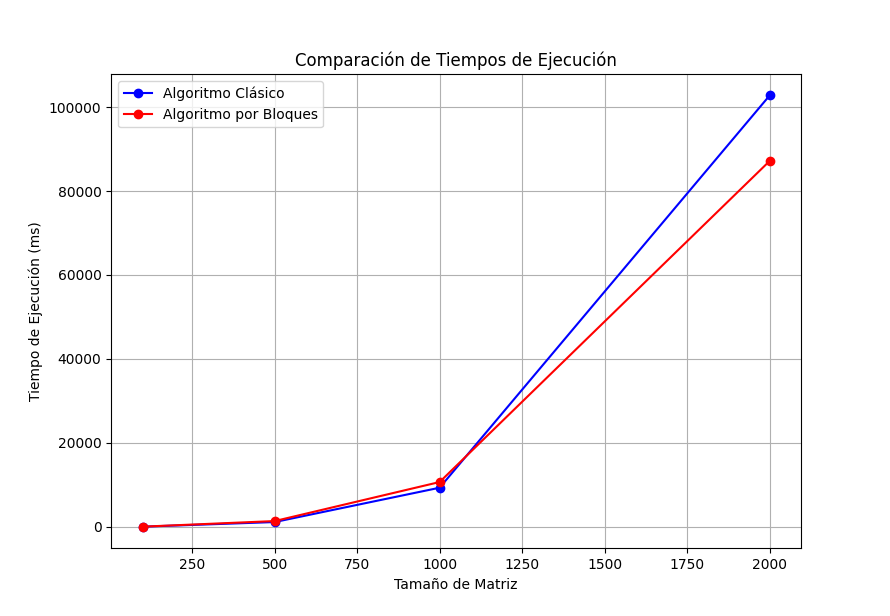
\includegraphics[width=\linewidth]{figures/grafico.png}
  \caption{Gráfico Comparativo }
  \label{fig:ec01}
\end{figure}

\section{Conclusiones}
\begin{itemize}
    \item Se puede visualizar una mayor diferencia entre los algoritmos mientras más grande es la matriz con la que se trabaja.
    \item Hay mejoras en los fallos de Caché de nivel 1 al reducir significativamente los fallos y mejorando el acceso a los datos.
    \item Se refleja una eficiencia superior en el uso del Caché al haber mejoras en los fallos de Caché de nivel 1 y último nivel usando la técnica de bloques.
    \item En general, la multiplicación de matrices por bloques demuestra ser superior a la clásica en la mayoría de las métricas de desempeño relacionadas con la caché. La reducción de fallos de caché y la mejora en la eficiencia del acceso a datos son evidentes, lo que sugiere que la técnica de bloques es más eficiente para matrices grandes y complejas
    \item Estas conclusiones destacan que la multiplicación de matrices por bloques no solo mejora el rendimiento en términos de acceso a caché, sino que también optimiza el uso de los recursos de memoria, resultando en un desempeño global más eficiente en comparación con el método clásico.
\end{itemize}

\begin{thebibliography}{9}

\bibitem{geeksforgeeks}
    GeeksforGeeks,
    \textit{Matrix Multiplication},
    \href{https://www.geeksforgeeks.org/matrix-multiplication/}{https://www.geeksforgeeks.org/matrix-multiplication/}

\bibitem{valgrind}
    Valgrind,
    \textit{Valgrind User Manual},
    \href{https://valgrind.org/docs/manual/index.html}{https://valgrind.org/docs/manual/index.html}

\bibitem{kcachegrind}
    KCachegrind,
    \textit{KCachegrind Documentation},
    \href{https://kcachegrind.sourceforge.net/html/Documentation.html}{https://kcachegrind.sourceforge.net/html/Documentation.html}

\bibitem{matrices}
    Lemat,
    \textit{Teoría sobre Multiplicación de Matrices},
    \href{https://www.lemat.unican.es/lemat/proyecto_lemat/matrices/nivel3/teoria/matrices8.htm}{https://www.lemat.unican.es/lemat/proyecto_lemat/matrices/nivel3/teoria/matrices8.htm}
\end{thebibliography}

\end{document}